%!TEX root = ../thesis.tex
\chapter{基于RGB-D图像的目标检测算法}
\label{chap:detector}
本章主要介绍所提出的两种基于RGB-D图像的目标检测算法3D Faster R-CNN和3D Mask R-CNN。3D Faster R-CNN是在Faster R-CNN\cite{Ren}的基础上,通过引入深度图以解决单从RGB图难以检测缺少纹理物体(Textureless Object)的问题,并且还引入了Spatial Transformer结构使得提取的特征具有旋转不变性。由于3D Faster R-CNN目标检测的结果是框出目标的Bounding Box,因此使得一些框住细长目标的Bounding Box内大部分像素并不属于该目标,这就使得后面的点云匹配算法难以得到满意的结果。因此3D Mask R-CNN根据Mask R-CNN\cite{He2017}对Faster R-CNN的改进思路,对3D Faster R-CNN进行了改进,使得其不仅能得到目标的Bounding Box,还能得到目标的Mask(可以知道Bounding Box内属于检测目标的像素),大大减少了后续匹配算法的难度。

\section{3D Faster R-CNN}
3D Faster R-CNN算法的整体结构如图\ref{fig:3d_faster_rcnn}所示。
\begin{figure}
  \centering
  todo:figure of 3d faster rcnn
  \caption{3D Faster R-CNN结构}
  \label{fig:3d_faster_rcnn}
\end{figure}

相比于Faster R-CNN,本文所提出的3D Faster R-CNN主要增加对深度信息的处理和Spatial Transformer,分别用于解决Faster R-CNN在实际应用时所不能解决的问题:
\begin{itemize}
\item 难以检测出缺少纹理的物体
\item 对物体的旋转敏感,提取的特征不具有旋转不变性
\end{itemize}

对于缺少纹理的物体,单从RGB图中很难检测出目标,这是一个很显然的问题,但是现在我们可以从对偶RGB-D相机中获取深度图,对于纹理少的物体,可以从深度图中提取特征检测出目标,所以现在的关键问题是如何从深度图中提取特征,并结合到Faster R-CNN中,本文所提出的方法是将深度图转换到HHA,然后再使用CNN提取特征,具体后文会详细介绍。

Faster R-CNN对于物体旋转敏感的问题,归根到底是因为CNN所提取的特征不具有旋转不变性,实际出现这种问题的情况,如图\ref{fig:cat}所示,
\begin{figure}[!ht]
  \centering
  \subfloat[检测旋转前的图片]{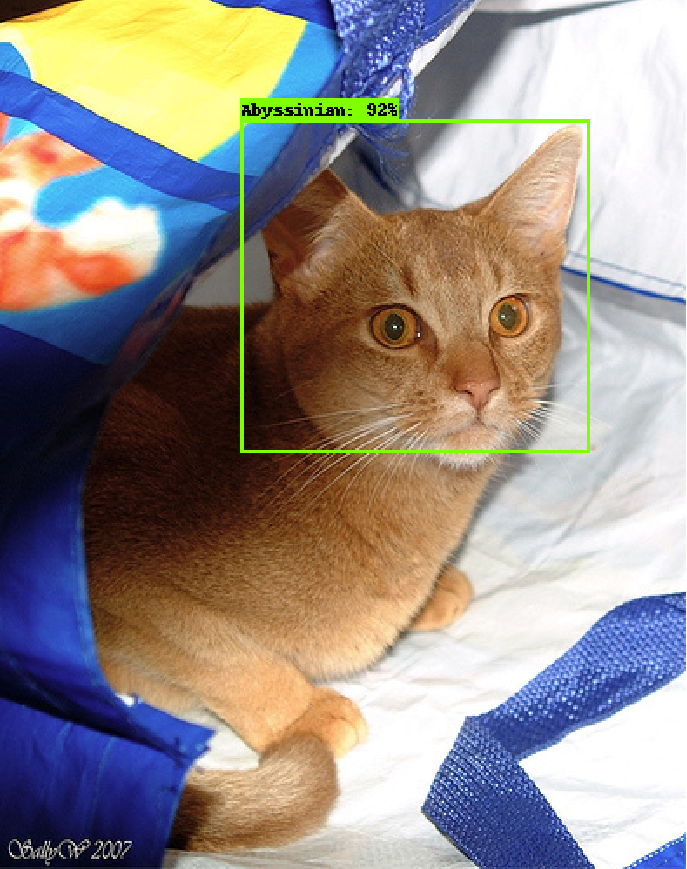
\includegraphics[width=4cm]{cat_up}}
  \hskip1em
  \subfloat[检测旋转后的图片]{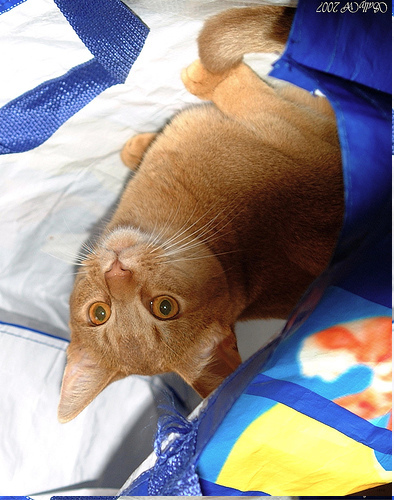
\includegraphics[width=4cm]{cat_down}}
  \caption{Faster R-CNN检测识别宠物猫示例}
  \label{fig:cat}
\end{figure}
其中图(b)只是将图(a)旋转了180度,由于CNN所提取的特征不具有旋转不变性,并且训练所实验的图片中的宠物都是头朝上的,即使图(a)在训练集中,将其旋转180度后,也无法从中检测出目标来。解决这个问题有两个思路:
\begin{itemize}
\item Data Augmentation
\item Spatial Transformer
\end{itemize}
Data Augmentation是通过对训练集中的图片进行旋转以获取不同角度的图片,通过这种方式增大数据集从而使得最终训练得到的模型对各种角度的图片都能识别;Spatial Transformer是一种特殊的网络结构,本文所使用的就这种方式,后文会详细介绍。

\subsection{Faster R-CNN}
为了更好地介绍所提出的3D Faster RCNN算法,先回顾一下Faster R-CNN算法。Faster R-CNN的网络结构如图\ref{fig:faster_rcnn}所示,
\begin{figure}
  \centering
  todo: faster rcnn 结构
  \caption{Faster R-CNN结构}
  \label{fig:faster_rcnn}
\end{figure}
Faster R-CNN的由两个核心模块构成:
\begin{itemize}
\item RPN(Region Proposal Network)
\item Fast R-CNN
\end{itemize}
整个网络是一个端到端(end-to-end)的目标检测网络,输入图片,输出图片中检测到的目标的类别和Bounding Box。RPN模块输出候选框,形象地说,RPN模块告诉Fast R-CNN模块去哪里检测目标,Fast R-CNN模块输出检测结果。

TODO:更详细的介绍?

\subsection{HHA}
有了与彩色图对应的深度图,如何有效地利用深度图是一个值得思考的问题。从2012年AlexNet\cite{Krizhevsky2012}在ImageNet\cite{imagenet}数据集上的应用开始,深度学习在计算机视觉领域其准确率相比传统方法有了一个很大的提升,因此,本文考虑通过深度学习的方法结合深度图和彩色图进行目标检测。深度学习在彩色图上的应用已经相当成熟,但对于深度图的应用还比较少,如何使用CNN在深度图上提取特征也是一个值得探讨的问题,是将深度图直接作为一个通道使用CNN提取特征?还是将深度图变换到三维坐标(x,y,z),然后再在这三个通道上通过CNN提取特征?经过实验和相关调研,发现将深度图转换为HHA图后进行训练的模型有较高的准确率\cite{Gupta2014},因此本文将深度图转换为HHA三个通道,然后再通过CNN提取特征。HHA三个通分别为:
\begin{itemize}
\item 水平方向上视差(Horizontal disparity)
\item 距离地面的高度(Height above ground)
\item 法向量与重力的夹角(Angle with gravity)
\end{itemize}
\textbf{Horizontal disparity:}深度图到视差的转换相对来说十分简单,理论上视差与深度呈倒数关系,因此水平方向上的视差计算具体如算法\ref{alg:hd}所示。
\begin{algorithm}[!ht]
  \caption{计算水平方向上视差}
  \label{alg:hd}
  \KwIn{Depth Frame $D_{h\times w}$}
  \KwOut{Horizontal disparity Frame $H_{h\times w}$}
  $h_{floor} = 1 / d_{ceil}, h_{ceil} = 1 / d_{floor}$\;
  \For {$y\leftarrow 1$ \KwTo $h$} {
    \For {$x\leftarrow 1$ \KwTo $w$} {
      $H[y, x] = 1 / D[y, x]$\;
      $H[y, x] = (H[y, x] - h_{floor}) / (h_{ceil} - h_{floor})$\;
    }
  }
\end{algorithm}

\textbf{Height above ground:}计算距离地面的高度首先要确定一个世界坐标系,然后得到世界坐标系到相机坐标系的旋转矩阵$\prescript{W}{C}{R}$和平移向量$\prescript{W}{C}{T}$,最后通过坐标变换得到距离地面的高度,具体如算法\ref{alg:hg}所示。
\begin{algorithm}[!ht]
  \caption{计算距离地面的高度}
  \label{alg:hg}
  \KwIn{Point Cloud $P_{h\times w}$}
  \KwOut{Hight Frame $H_{h\times w}$}
  \For {$y\leftarrow 1$ \KwTo $h$} {
    \For {$x\leftarrow 1$ \KwTo $w$} {
      $p =  \prescript{W}{C}{R}P[y, x] + \prescript{W}{C}{T}$\;
      $H[y, x] = p.z$\;
    }
  }
\end{algorithm}

\textbf{Angle with gravity:}法向量与重力的夹角的计算相对来说稍微复杂一点,重力的方向在工作区间内一般与所设的世界坐标系的$z$轴负方向相同,因此原问题就是求法向量与世界坐标系$z$轴负方向之间的夹角。参考文献\cite{Gupta2013},首先计算深度图中每个点上的法向量,具体如算法\ref{alg:normal}所示。
\begin{algorithm}[!ht]
  \caption{计算法向量}
  \label{alg:normal}
  todo: normal algorithm\;
  \KwIn{Point Cloud $P_{h\times w}$}
  \KwOut{Hight Frame $H_{h\times w}$}
  \For {$y\leftarrow 1$ \KwTo $h$} {
    \For {$x\leftarrow 1$ \KwTo $w$} {
      $p =  \prescript{W}{C}{R}P[y, x] + \prescript{W}{C}{T}$\;
      $H[y, x] = p.z$\;
    }
  }
\end{algorithm}



\subsection{Spatial Transformer}


\section{3D Mask RCNN}

\section{目标检测实验}

\section{本章小结}

